\documentclass[article]{jss}
\usepackage{thumbpdf,lmodern} 
\graphicspath{{Figures/}}

\usepackage{amsmath}

\author{Joke Durnez\\ Stanford University and INRIA \And
        Ross Blair\\ Stanford University \And
        Russell A. Poldrack \\ Stanford University}

\title{\pkg{neurodesign}: Optimal Experimental Designs for Task fMRI}

\Abstract{ A recent stream of alarmist publications has questioned the
  validity of published neuroimaging findings.  As a consequence, fMRI
  teams worldwide have been encouraged to increase their sample sizes
  to reach higher power and thus increase the positive predictive
  value of their findings.  However, an often-overlooked factor
  influencing power is the experimental design: By choosing the
  appropriate experimental design, the statistical power of a study
  can be increased within subjects.  By optimizing the order and
  timing of the stimuli, power can be gained at no extra cost.
  
  To facilitate design optimization, we created a \proglang{Python}
  package and web-based tool called \pkg{neurodesign} to maximize the
  detection power or estimation efficiency within subjects, while
  controlling for psychological factors such as the predictability of
  the design.  We implemented both a simulation-based optimization, as
  well as an optimization using the genetic algorithm, introduced by
  \citet{Wager2003-hy} and further improved by \citet{Kao2009-yo}, to
  optimize the experimental design.  The toolbox \pkg{neurodesign}
  allows more complex experimental setups than existing toolboxes,
  while the graphical user interface (GUI) provides a more
  user-friendly experience.  The toolbox is accessible online at
  \url{http://www.neuropowertools.org}.  }

\Keywords{fMRI, experimental design, \proglang{Python}, GUI, statistical power}
\Plainkeywords{fMRI, experimental design, Python, GUI, statistical power}

\Address{
  Joke Durnez\\
  Department of Psychology\\
  Stanford University\\
  560 Serra Mall\\
  Stanford, CA 94305\\
  E-mail: \email{joke.durnez@gmail.com}\\
  URL: \url{http://www.neuropowertools.org}
}


\begin{document}

\section{Introduction}\label{sec:introduction}
A recent stream of alarmist publications has questioned the validity
of published neuroimaging findings
\citep{Eklund2016-il,Ioannidis2005-ls,Open_Science_Collaboration2015-ev}.
At the core of the reproducibility crisis is the lack of power
typically observed in neuroimaging \citep{Button2013-zr}, and more
specifically, fMRI studies \citep{Durnez2014-ev}.  The signal measured
in fMRI is known to be very noisy, while the hypothesized effects are
small, such that a push for larger sample sizes promises a more
powerful future for neuroimaging.  Different power analysis strategies
offer a way to optimize the sample size for a specific power level
\citep{Durnez2014-ev,Mumford2008-qu,Hayasaka2007-fh,Durnez2016-bn}.
However, fMRI data are typically acquired and aggregated on two
levels: within and between subjects.  As such, increasing the power of
an fMRI experiment can be achieved by increasing the number of
subjects, but also via the within-subjects experimental design.  This
is especially true for smaller and more subtle effects, where the
power curve is characterized by a slower increase, and thus the
resulting power is more affected by the number of subjects and the
number of time points.  In addition to the duration of the experiment
for each subject, the order and timing of different conditions within
the experiment also influence the power of the resulting analyses.

The goal in task fMRI experiments is often one of two: detection or
estimation.  Detection refers to detecting the difference in brain
activation between conditions or groups, while estimation relates to
estimating the exact shape of the evoked fMRI response (called the
hemodynamic response function, HRF).  Ideally, the design of an fMRI
experiment changes according to the specific research question asked.
An optimal design with respect to these two distinct research
questions are said to maximize the detection power or the estimation
efficiency respectively.  It is often argued that those two goals are
opposite and an increase in detection power inevitably leads to a
decrease of estimation efficiency.  For example, when two trials of
the same condition follow each other closely, the signal tends to
accumulate linearly \citep{Dale1999-ik}, which makes it easier to
detect.  Therefore, the experiments often consist of blocks of the
same condition.  This type of design is called a blocked design.  On
the contrary, the accumulation (and saturation) of the measured signal
conceals the shape of the HRF.  To estimate the HRF, scientists often
opt for an event-related design, where both the timing and order of
conditions are randomized.  However, \citet{Kao2009-yo} show that the
necessary trade-off between detection and estimation can be improved
using certain optimization algorithms.

Another important aspect in an fMRI design is the psychological
experience of the subject in the scanner. With a blocked design, the
design becomes very predictable for subjects which can potentially
bias the psychological function under investigation.  To minimize
predictability, \citet{Buracas2002-sg} propose the use of $m$-sequences.
However, the length of an $m$-sequence is restricted to $n=(Q_1)^l -1$ with
$Q+1$ a prime, $Q$ the total number of stimulus types, and $l$ a
positive nonzero integer.  Recently \citet{Lin2007} proposed the use
of a circulant (almost-)orthogonal array to expand the range of
possible fMRI designs while ensuring complete independence between a
trial and its successor.  Very often, the best design is a combination
of a maximal signal with low predictability.  Therefore,
\citet{Wager2003-hy} suggest the use of a genetic algorithm to find an
optimization between estimation efficiency, detection power and
predictability.  This algorithm optimizes a weighted average of
different criteria, with the weights depending on the hypothesis and
the expected outcome of the experiment.  Subsequent work has further
fine-tuned the algorithm and compared it with other approaches
\citep{Kao2009-yo}.  However, in some cases the design requires more
control than is offered in the genetic algorithm, in which case a
simulation-based optimization is the only considerable option.  In
this paper, we present \pkg{neurodesign} for fMRI design optimization
with different optimization algorithms, which is both available as a
\proglang{Python} \citep{python} module as well as a GUI web tool, available at
\url{http://www.neuropowertools.org}.  The paper is structured as
follows: We start with a general description of the methodology in
Section~\ref{sec:design-optim-using}.  We show how designs can be
compared and optimized using our \proglang{Python} module in
Section~\ref{sec:pkgn-progl-module}.  An overview of the GUI is given
in Section~\ref{sec:pkgneurodesign:-gui}.  We compare our toolbox with
other existing software in Section~\ref{sec:comp-with-other} and
compare the designs from different optimizers in
Section~\ref{sec:design-optim-stat}.  Finally, we conclude and discuss
the results in Sections~\ref{sec:discussion} and \ref{sec:conclusion}.

\section{Design optimization using the genetic algorithm}\label{sec:design-optim-using}

\subsection{Statistical measures of design optimality}

The signal measured using fMRI is the blood oxygen level dependent
(BOLD) signal, which is a assumed to be related to the neural signal
via convolution with a hemodynamic response function (HRF).  We
consider the general linear model (GLM) as the underlying model for
the statistical objective as in Equation~\ref{eq:GLM}.
%
\begin{equation} \label{eq:GLM}
Y = X\beta + \epsilon, \epsilon \sim N(0,\sigma^2)
\end{equation}
%
We denote  $Y$  as the measured signal.  $X$ represents the design matrix,  $\beta$  is the response amplitude for each column/condition in $X$ and $\epsilon$ the error.

There are two types of design matrices: the convolved model and the
finite impulse response (FIR) model where both are transformations of
the matrix $X_\text{base}$, an $m \times t$ matrix, where $m$ is the
number of stimuli and $t$ the number of measured time points.  The
values in $X_\text{base}$ are 1 or 0: 1 when stimulus $M$ is shown on
time point $T$.  The two transformations of $X$ are shown in
Figure~\ref{fig1}.  In the first model, the regressor $X_\text{base}$
is convolved with the hemodynamic response function (Figure~\ref{fig1},
panel 2) to represent the expected signal for a brain region related
to the stimulus.  The second model aims to estimate the exact shape of
the HRF, by including regressors identical to the stimulus
presentation, but each regressor with a certain temporal lag
(Figure~\ref{fig1}, panel 3).
%
\begin{figure}[t!]
\centering
1. \\
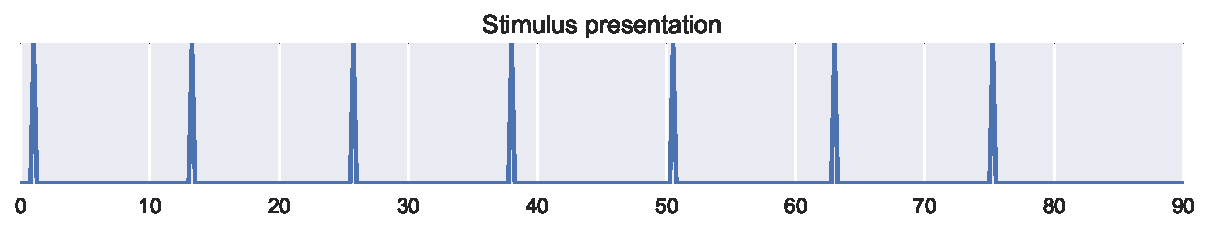
\includegraphics[scale=2]{Figure1a.pdf} \\
2. \\
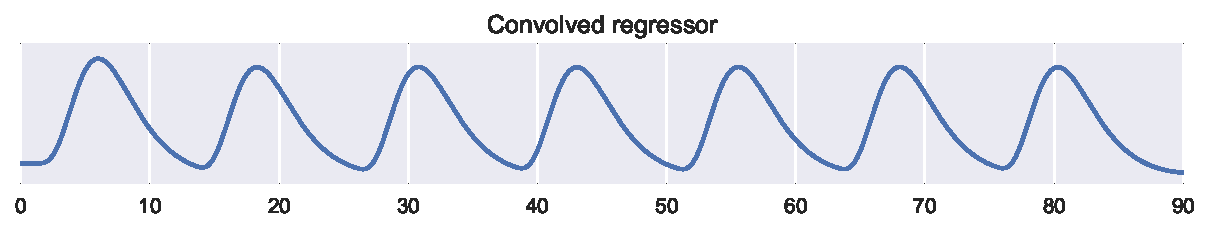
\includegraphics[scale=2]{Figure1b.pdf} \\
3. \\
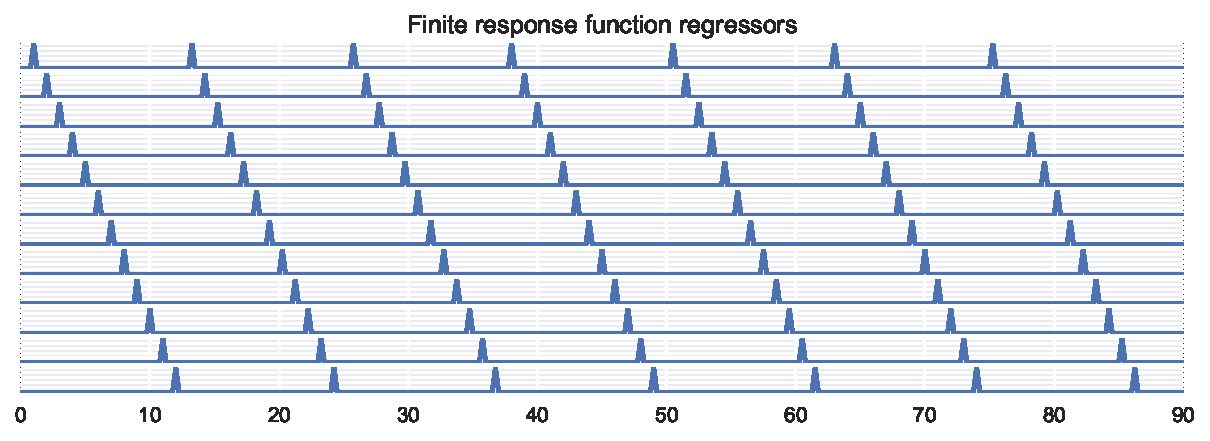
\includegraphics[scale=2]{Figure1c.pdf}
\caption{An experimental fMRI design with one stimulus type and two
  common models used in the GLM when modeling the resulting BOLD
  signal.  The first panel shows the time series of the stimulus
  onsets.  The second panel shows the stimulus onsets convolved with
  the double-gamma HRF, which can be interpreted as the expected BOLD
  signal if the measurement is related to the task.  The parameter
  $\beta$ in Equation~\ref{eq:GLM} represents the amplitude of the
  signal related to the task. The third panel shows the FIR model,
  with each regressor a shifted version of the stimulus onsets.  The
  parameter $\beta$ represents the amplitude of the HRF at specific
  time points following stimulus onset.  Units on the $x$-axis are
  seconds.  Units on the $y$-axis are removed, as these are
  meaningless and often rescaled to have unit height.\label{fig1}}
\end{figure}

Often, researchers are interested in specific hypotheses concerning
particular combinations of parameters.  The parameter of interest
$\beta$ can be estimated using the least squares estimator in
Equation~\ref{eq:LSE} and its variance in Equation~\ref{eq:var}.%
\begin{align}
\hat\beta_c &= c^\top(X^\top X)^{-1}X^\top Y \label{eq:LSE}\\
\VAR(\hat\beta_c) &= \sigma^2c(X^\top X)^{-1}c^\top \label{eq:var}
\end{align}
with $c$ the contrast vector of interest.  To account for the specific
character of fMRI data, we alter the model slightly.  Because fMRI
time series data exhibit substantial temporal autocorrelation, the
errors in Equation~\ref{eq:GLM} are not independent, $\epsilon \sim N(0, \sigma^2V)$,
where off-diagonal values represent the correlation between
measurements at different time points.  Furthermore a regressor, $S$,
representing low-frequency noise components is added to the model (see
\citealt{Kao2009-yo} for detailed derivations).  The resulting
variance of the estimator in defined in Equation~\ref{eq:varest}.
%
\begin{equation} \label{eq:varest}
\VAR(\hat\beta_c) = \sigma^2c(X^\top WX)^{-1}c^\top
\end{equation}
%
with $W = V-VS^\top(SVS^\top)^{-1}SV$.  An optimal experimental design with respect to the estimator minimizes the variance of the estimator. We will therefore quantify the optimality of the design as the inverse of $c(X^\top WX)^{-1}c^\top$.  Most often, an fMRI experiment has multiple contrasts of interest,  thus $c(X^\top WX)^{-1}c^\top$ becomes a square matrix.  With $r_c$ the number of contrasts, there are two common ways to quantify the optimality of the design as defined in Equation~\ref{eq:opt}.
%%
\begin{equation}%
\begin{aligned}\label{eq:opt}
F &= r_c/\text{trace}(C(X^\top WX)^{-1}C^\top)  \text{ for A optimality} \\
F &= \det(C(X^\top WX)^{-1}C^\top)^{-1/r_c} \text{ for D optimality}
\end{aligned}
\end{equation}
%
We denote $F_e$ as the estimation efficiency if $X$ is a FIR, and $F_d$ as the detection power if $X$ is a convolved design matrix.

\subsection{Psychological measures of design optimality}

Apart from the statistical concept of design efficiency, it is important to account for psychological factors that might render the experimental design invalid.  The most important factor is predictability.  For example in experiments addressing cognitive control, such as a stop-signal task, it is of the utmost importance that the trial type on any given trial cannot be easily predicted from the trial type on the previous trial, to avoid psychological confounding of the experiment.  We quantify the optimality of the design in terms of confounding in Equation~\ref{eq:confounding}.
%%
\begin{equation} \label{eq:confounding}
F_c = \sum_{r=1}^R \sum_{i=1}^Q \sum_{j=1}^Q {n_{ij}^{r}-(n-r)P_iP_j },
\end{equation}
%
where $n_{ij}^r$ is the number of trials of type $i$ at time point $t$
preceding a trial of type $j$ at time point $t+r$.  The variable $P_i$
is the proportion that this trial should occur in the experiment.  If
$F_c=0$, there are no unforeseen contingencies between trial types.
The final optimality criterion controls the desired trial type
frequencies: $F_f = \sum_{i=1}^Q | n_i-nP_i | $, with $n_i$ the number
of trials of type $i$.

\subsection{Multi-objective criterion}

To ensure comparability across different optimality criteria, we first
rescale the different optimality criteria to a scale of 0 to 1 as in
\citet{Kao2009-yo}.  To find the maximum $F_d$ and $F_e$ possible, we
first run an optimization with weights 1 for respectively $F_d$ and
$F_e$ and weights 0 for the other optimality criteria.  In the
multi-objective criterion, the $F_d$ and $F_e$ scores are divided by
their respective maximum to ensure scores between 0 and 1.  For $F_f$
and $F_c$, the score for the worst possible design (a design with only
the least probable stimulus) is taken as the maximum score.  Second,
whereas larger $F_e$ and $F_d$ represent better designs, the opposite
is true for $F_c$ and $F_f$.  Therefore the scores for $F_c$ and $F_f$
are subtracted from 1.  As such, the resulting optimality criterion is
obtained in Equation~\ref{eq:optim}.
%
\begin{align} \label{eq:optim}
  F_i^* &= \left\{
\begin{array}{ll}
  \frac{F_i}{\max(F_i)},& i=d,e \\
  1-\frac{F_i}{\max(F_i)},&i=c,f
\end{array}\right.                            
\end{align}
%
As no design can ensure optimality in all four optimality criteria, the goal of any design optimization depends on the researcher's goal of the experiment.  Given prespecified weights $w_i$ with $i=c,d,e,f, \sum_iw_i=1,w_i\geq0$, we define the weighted optimality criterion in Equation~\ref{eq:weighted}.
%
\begin{equation}\label{eq:weighted}
F^*= w_cF_c + w_dF_d + w_eF_e + w_fF_f
\end{equation}
%
\subsection{Optimization algorithms}

\subsubsection{Genetic algorithm}

A genetic algorithm is a method for solving optimization problems
inspired by natural selection in biological evolution.  Contrary to
classical optimization algorithms, a genetic algorithm generates a
population of points at each iteration.  A graphic representation of
the genetic algorithm with an fMRI example is shown in
Figure~\ref{fig2}.  The steps of the genetic algorithm are.
%
\begin{enumerate}
 \setlength\itemsep{-0.5em}
\item Create $G$ initial random designs.
\item \textbf{Crossover.} Pair the best $G$/2 designs with each other.
\item \textbf{Mutation. }Randomly switch $q$\% of all trials by random trial types.
\item \textbf{Immigration.} Add new random designs to the population.
\item \textbf{Natural selection.}  Compute optimality scores and select $G$ best designs.
\item Repeat steps 2--5 until a stopping rule is met.
\end{enumerate}

A crucial part of the algorithm is drawing random designs from the
population of designs (in step 1 and step 4).  This could for example
be achieved by using $m$-sequences to decide the order of the stimuli,
the stimuli evenly spaced in time.  We show in
Section~\ref{sec:gener-rand-design} how to sample random designs using
\pkg{neurodesign}.
%
\begin{figure}[t!]
\centering
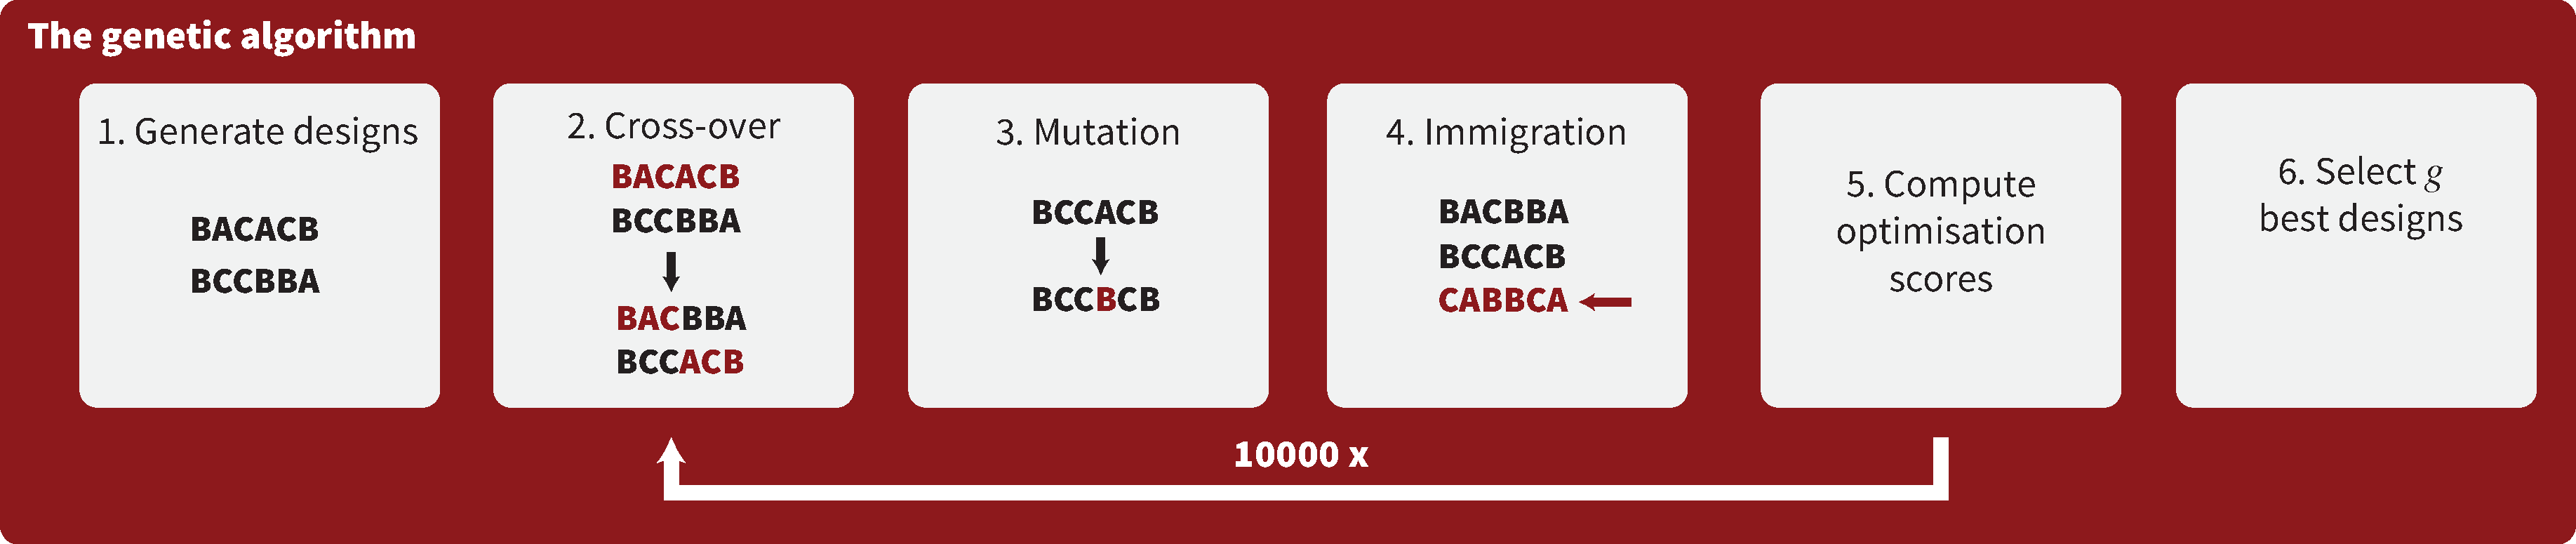
\includegraphics[scale=0.5]{GA.pdf}
\caption{Graphical representation of the genetic algorithm.  The examples in each step are pieces of experimental designs with 3 different trial types (A, B, C).  In the example, the inter-trial interval is ignored. \label{fig2}}
\end{figure}


\subsubsection{Simulation-based optimization}

While the genetic algorithm has been shown to be a powerful algorithm
for experimental design optimization \citep{Kao2009-yo}, there are
certain instances where more strict control of the design is desired.
For example, in cognitive control, the occurrence of one condition
versus another is sometimes varied between subjects.  In those
instances, it is crucial that there is strict control of the
proportion of trial types that are shown.  The genetic algorithm
punishes deviance from the proportions measured by $F_f$, but strict
control cannot be ensured.  Therefore, we included a random design
generator.  The implementation is identical to the \textit{genetic
  algorithm}, with the \textit{crossover}- and \textit{mutation}-steps
removed and only the \textit{immigration}-step being performed.

\section[Python module neurodesign]{\proglang{Python} module \pkg{neurodesign}}\label{sec:pkgn-progl-module}

\subsection{Installation}\label{sec:installation}

\pkg{neurodesign} is available on PyPi and can be installed as:
%
\begin{CodeChunk}
\begin{CodeInput}
$ pip install neurodesign
\end{CodeInput}
\end{CodeChunk}
%
Next, we will give an introduction to the \proglang{Python} module.  For all functionality, please refer to the manual.

\subsection{Specifying the characteristics of the experiment}

In a first step, the experiment should be described in the class
called `\code{experiment}'.  This contains general information, such
as the number of stimuli and the duration of the experiment, but also
more specific information, such as the model with which the inter
trial intervals (ITI) are sampled.  This function will generate the
assumed covariance matrix, the drift function and the whitening
matrix.  All parameters are described in Table~\ref{experiment}, while
a graphical representation of components of an experiment are
described in Figure~\ref{fig3}.  We define a simple experimental setup
with 20 trials and 3 conditions, which we will use to exemplify the
next functions:
%%
\begin{CodeChunk}
\begin{CodeInput}
>>> import neurodesign
>>> EXP = neurodesign.experiment(TR = 1.2, n_trials = 20, 
...   P = [0.3, 0.3, 0.4], C = [[1, -1, 0], [0, 1, -1]], n_stimuli = 3,  
...   rho = 0.3, stim_duration = 1, ITImodel = "uniform", ITImin = 2, 
...   ITImax = 4)
\end{CodeInput}
\end{CodeChunk}
%%
\begin{figure}[t!]
\centering
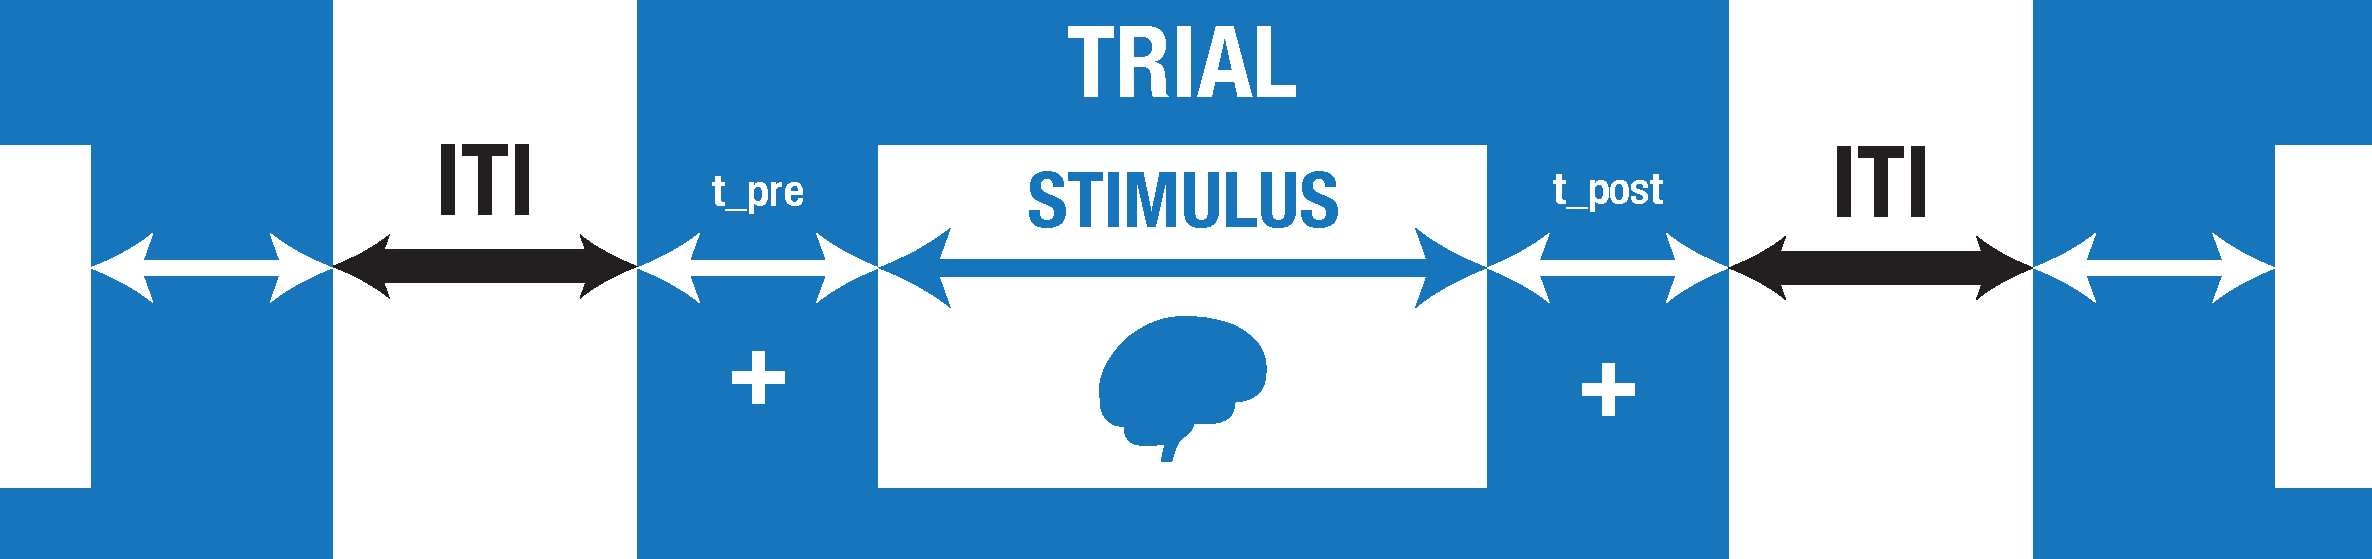
\includegraphics[scale=0.35]{experiment_structure.pdf}
\caption{The basic layout of an experimental trial. \label{fig3}}
\end{figure}
%
\begin{table}[t!]%
  \centering
  \begin{tabular}{lp{9.5cm}}
\hline
Argument&Description\\   
\hline    
\code{TR} &
The repetition time of the scanner.\\
\code{n\_stimuli}  &
The number of different stimulus types or conditions.\\
\code{P} &
The probabilities of each stimulus type.\\
\code{C} &
The contrast matrix.\\
\code{rho} &
The assumed autocorrelation coefficient.\\
\code{n\_trials} &
The number of trials in the experiment.  Either specify \code{n\_trials} \emph{or} \code{duration}. \\
\code{duration}&
The total duration (seconds) of the experiment.  Either specify \code{duration} \emph{or} \code{n\_trials}. \\
\code{resolution} (default = 0.1) &
The resolution of the design matrix. \\
\code{t\_pre} (default = 0) &
Duration (seconds) of the trial before the stimulus presentation (e.g., fixation cross). \\
\code{stim\_duration} &
The duration (seconds) of the stimulus. \\
\code{t\_post} (default = 0) &
Duration (seconds) of the trial after the stimulus presentation. \\
\code{maxrep} (default = \code{None}) &
The maximum number of times a stimulus is repeated consecutively. \\
\code{hardprob} (default = \code{False}) &
\code{True} if the probabilities should be exactly the same as in \code{P}. \\
\code{restnum} (default = 0) &
The number of trials between rest blocks. \\
\code{restdur} (default = 0) &
The duration (seconds) of a rest block. \\
\code{ITImodel} &
Which ITI model to sample from.  Possibilities: \code{"fixed"}, \code{"uniform"} or \code{"exponential"}. \\
\code{ITImin} &
The minimum ITI (used with \code{"uniform"} or \code{"exponential"} ITImodel). \\
\code{ITImean} &
The mean ITI (used with \code{"fixed"} or \code{"exponential"} ITImodel). \\
\code{ITImax} &
The max ITI (used with \code{"uniform"} or \code{"exponential"} ITImodel). \\
\code{confoundorder} (default = 3) &
The order to which confounding is controlled. \\
\hline    
\end{tabular}
\caption{The arguments for an object of class `\code{neurodesign.experiment}'. \label{experiment}}
\end{table}

\subsection{Generating a design matrix}
Within the defined experimental setup, we can now define a design
matrix, develop the design matrix and compute the optimality scores
using the class `\code{design}'.  We use equal weights for the different
optimality criteria for the weighted average optimality attribute.
The only input required is the stimulus order, the ITI's and an object
of class `\code{neurodesign.experiment}':
%%
\begin{CodeChunk}
\begin{CodeInput}
>>> import neurodesign
>>> DES1 = neurodesign.design(
...   order = [0, 1, 2, 0, 1, 2, 0, 1, 2, 0, 1, 2, 0, 1, 2, 0, 1, 2, 0, 1],
...   ITI = [2] * 20, experiment = EXP)
>>> DES1.designmatrix(); DES1.FCalc(weights = [0.25, 0.25, 0.25, 0.25])
\end{CodeInput}
\end{CodeChunk}
%
Now using \pkg{matplotlib} \citep{matplotlib}, we can plot the
convolved design matrix (see Figure~\ref{fig:cov}):
%%
\begin{CodeChunk}
\begin{CodeInput}
>>> import matplotlib.pyplot as plt
>>> plt.plot(DES1.Xconv)
\end{CodeInput}
\end{CodeChunk}
%%
\begin{figure}[t!]
  \centering
  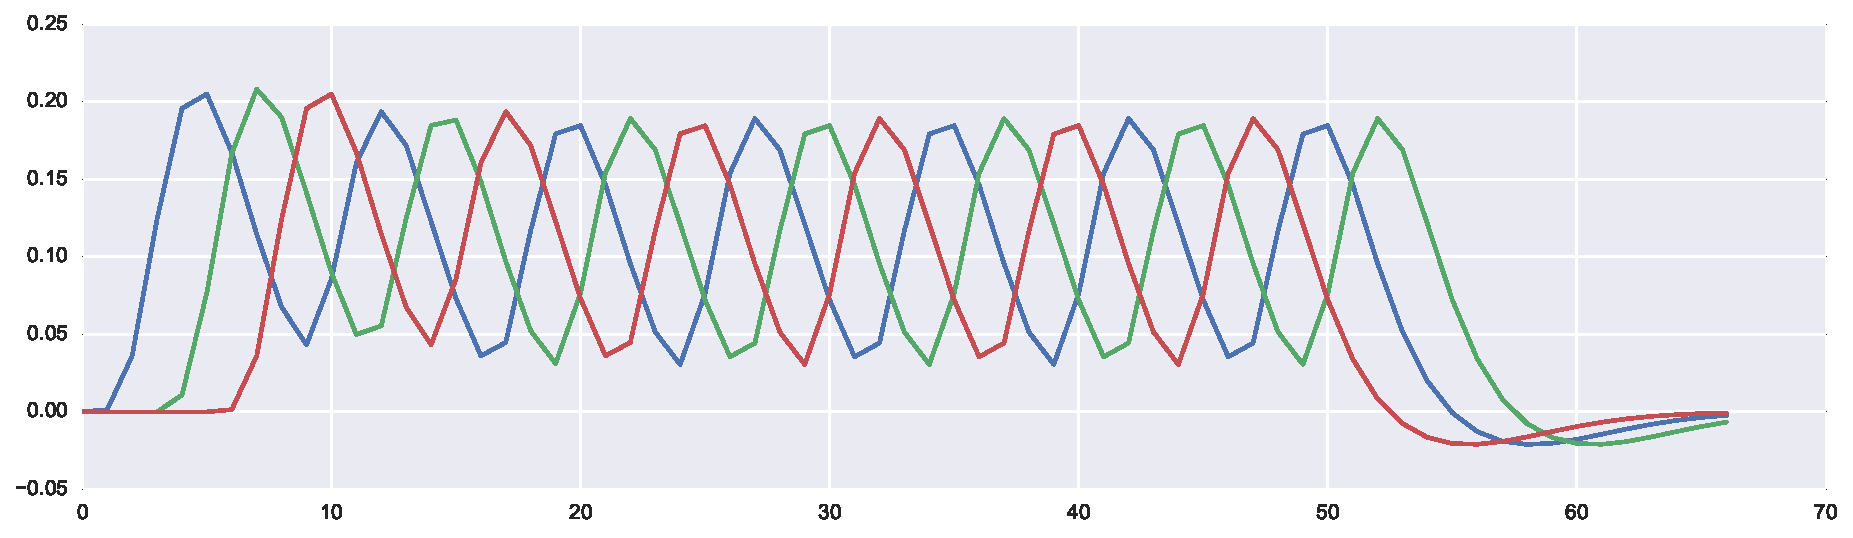
\includegraphics[scale=0.35]{Figure4.pdf}
  \caption{Plot of the convolved design matrix.\label{fig:cov}}
\end{figure}
We can now define a new design and compare both designs:
%%
\begin{CodeChunk}
\begin{CodeInput}
>>> DES2 = neurodesign.design(
...   order = [0, 0, 0, 0, 0, 1, 1, 1, 1, 1, 0, 0, 0, 0, 0, 1, 1, 1, 1, 1],
...   ITI = [2] * 20, experiment = EXP)
>>> DES2.designmatrix(); DES2.FCalc(weights = [0.25, 0.25, 0.25, 0.25])
>>> print("Ff of Design 1: "+str(DES1.Ff))
>>> print("Ff of Design 2: "+str(DES2.Ff))
>>> print("Fd of Design 1: "+str(DES1.Fd))
>>> print("Fd of Design 2: "+str(DES2.Fd))
\end{CodeInput}
\begin{CodeOutput}
Ff of Design 1: 0.8571428571428572
Ff of Design 2: 0.4285714285714286
Fd of Design 1: 0.0879554751884
Fd of Design 2: 0.266229261071
\end{CodeOutput}
\end{CodeChunk}
%
As the second design ignores the presence of the third condition, the
frequency optimality ($F_f$) is much worse.  However, the blocked
character of the design largely improves the detection power.  The
principles of the genetic algorithm, such as crossover, can be applied
to the designs:
%%
\begin{CodeChunk}
\begin{CodeInput}
>>> DES3,DES4 = DES1.crossover(DES2, seed = 2000)
>>> DES3.order
\end{CodeInput}
\begin{CodeOutput}
[0, 1, 2, 0, 1, 2, 0, 1, 1, 1, 0, 0, 0, 0, 0, 1, 1, 1, 1, 1]
\end{CodeOutput}
\begin{CodeInput}
>>> DES4.order
\end{CodeInput}
\begin{CodeOutput}
[0, 0, 0, 0, 0, 1, 1, 1, 2, 0, 1, 2, 0, 1, 2, 0, 1, 2, 0, 1]
\end{CodeOutput}
\end{CodeChunk}
%
\subsection{Generating a random design}\label{sec:gener-rand-design}

The package contains functions to generate random designs.  We can
generate a random order of stimuli using the function
\code{neurodesign.generate.order}.  Below, we generate a random order of
stimuli, which is done by sampling from a multinomial distribution.
Below, the resulting probabilities for each trialtype are shown.
%%
\begin{CodeChunk}
\begin{CodeInput}
>>> order = neurodesign.generate.order(nstim = 4, ntrials = 100,
...   probabilities = [0.25, 0.25, 0.25, 0.25], ordertype = "random",
...   seed = 1234)
print(order[:10])
from collections import Counter
Counter(order)
\end{CodeInput}
\begin{CodeOutput}
[3, 0, 0, 2, 0, 0, 2, 2, 2, 0]
Counter({0: 36, 1: 22, 2: 22, 3: 20})
\end{CodeOutput}
\end{CodeChunk}
%
Similarly, we can generate ITI's from 3 different distributions: fixed
(all ITI's equal), uniform or from a truncated exponential
distribution.  Below we show how to use and evaluate the output of
function \code{neurodesign.generate.iti}.
%%
\begin{CodeChunk}
\begin{CodeInput}
>>> iti,lam = neurodesign.generate.iti(ntrials = 40, model = "exponential",
...   min = 2, mean = 3, max = 8, resolution = 0.1, seed = 2134)
>>> print(iti[:10])
>>> print("mean ITI: %s \nmin ITI: %s \n max ITI: %s"
...   %(round(sum(iti)/len(iti), 2),
...   round(min(iti), 2), round(max(iti), 2)))
\end{CodeInput}
\begin{CodeOutput}
[0.  2.  2.1 2.  2.  2.  5.4 2.  2.4 5.1]
mean ITI: 2.93
min ITI: 0.0
max ITI: 6.9
\end{CodeOutput}
\end{CodeChunk}
%
\subsection{Optimizing the design}

To optimize the design, we use the `\code{neurodesign.optimization}'
class.  All parameters are described in Table~\ref{population}.
%%
\begin{CodeChunk}
\begin{CodeInput}
>>> POP = neurodesign.optimisation(experiment = EXP,
...   weights = [0, 0.5, 0.25, 0.25], preruncycles = 10000,
...   cycles = 10000, folder = "./", seed = 100, optimisation = "GA")
>>> POP.optimise()
\end{CodeInput}
\end{CodeChunk}
%%
\begin{table}[t!]%
  \centering
\begin{tabular}{lp{9.5cm}}
\hline
Argument&Description\\   
\hline    
\code{experiment} &
The experimental setup of the fMRI experiment (of class `\code{neurodesign.experiment}'). \\
\code{G} (default = 20) &
The size of each generation. \\
\code{R} (default = \code{[0.4, 0.4, 0.2])} &
The rate with which the orders are generated from (a) blocked designs, (b) random designs and (c) $m$-sequences. \\
\code{q} (default = 0.01) &
The percentage of mutations in each generation. \\
\code{weights} &
The weights attached to [$F_e$, $F_d$, $F_f$, $F_c$]. \\
\code{I} (default = 4) &
The number of immigrants in each generation. \\
\code{preruncycles} &
The number of pre-run cycles to find the maximum value of $F_e$ and $F_d$. \\
\code{cycles} &
The number of cycles in the optimization. \\
\code{seed} &
The random seed for the optimization. \\
\code{Aoptimality} (default = \code{True}) &
Optimizes A-optimality if \code{True}, else D-optimality. \\
\code{convergence} (default = 1000) &
After how many stable iterations is there convergence. \\
\code{folder} &
The local folder to save the output. \\
\code{outdes} (default = 3) &
The number of designs to be saved. \\
\code{optimization} (default = \code{"GA"}) &
                                               The optimizer of choice (\code{"GA"} or \code{"simulation"}).\\
\hline                                              
\end{tabular}
\caption{The arguments for an object of class `\code{neurodesign.optimisation}'. \label{population}}
\end{table}

\section[neurodesign: The GUI]{\pkg{neurodesign}: The GUI}\label{sec:pkgneurodesign:-gui}

To make the methods more publicly available, we have created a
graphical user interface running in a web application.  The back-end
of the application is written in \proglang{Python} and uses the
\proglang{Python} module \pkg{neurodesign} described above, the
front-end is generated using \pkg{django} \citep{django}, and the
application is deployed through a multi-container docker environment
on Amazon Web Services.

There are 5 crucial windows of the GUI: main input, contrasts and
probabilities, review, console, and settings.  The main input window
has fields for most parameters from Table~\ref{experiment}.  Only the
parameters $P$ and $C$ are asked in the second window (`Contrasts and
probabilities').  The review window shows all parameters and also
prints out the default settings for the genetic algorithm.  These
parameters, presented in Table~\ref{population}, can be adjusted in
the settings window.  The console allows for the optimizations to be
started, stopped and followed.  When a design optimization is started,
the user receives an email with a link to the console where the
optimization can be followed (Figure~\ref{fig6}). Once the
optimization is finished, a zip file can be downloaded containing a
chosen number of designs.  Each design contains the onsets for each
stimulus, a report with design diagnostics (such as collinearity among
regressors, see Figure~\ref{fig7}), and a script.  The script can be
used for future reference, or for regenerating the designs locally.
%
\begin{figure}[t!]
\centering
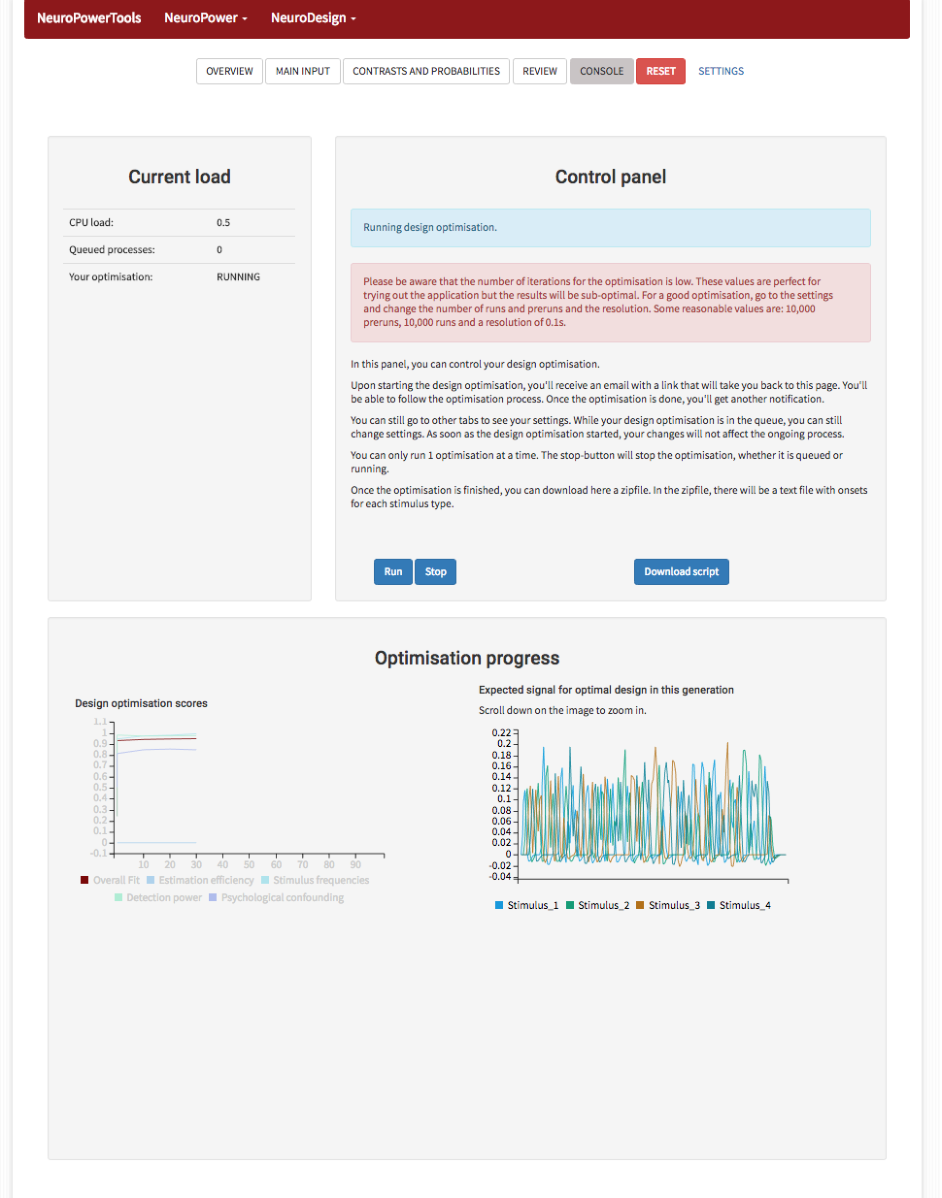
\includegraphics{screenshot2.pdf}
\caption{Screenshot of the console where the optimization can be followed.  Every 10 generations, the design is updated with the latest score and the best design.\label{fig6}}
\end{figure}
%
\begin{figure}[t!]
\centering
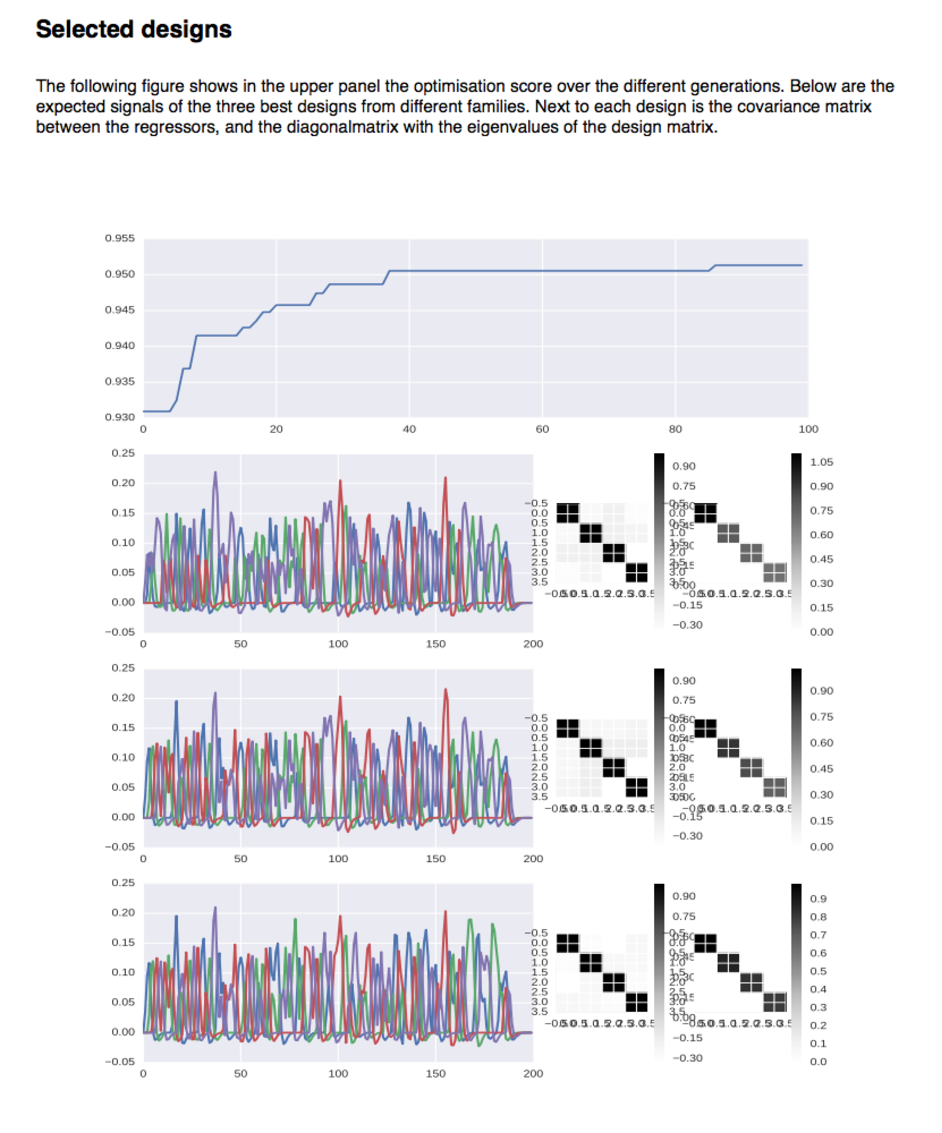
\includegraphics[trim = 0 10 0 10, clip]{screenshot3.pdf}
\caption{Screenshot of the report describing the optimization and the best 3 designs from the optimization.\label{fig7}}
\end{figure}

\section{Comparison with other software}\label{sec:comp-with-other}

There are a few alternative design optimization programs available:

\subsubsection[mseq]{\code{mseq}}
This function, available in the script
\url{http://gru.stanford.edu/svn/matlab/buracas.m} was distributed
with \citet{Buracas2002-sg} and can be used to generate $m$-sequences
using \proglang{MATLAB} \citep{MATLABR2019a}.

\subsubsection[riksneurotools]{\pkg{riksneurotools}}
The tool \pkg{riksneurotools} is provided by \citet{Henson2006} to
compute the GLM efficiency of experimental designs for fMRI in
\proglang{MATLAB} and is available online at
\url{https://github.com/MRC-CBU/riksneurotools}.

\subsubsection[mttfmri toolbox]{\pkg{mttfmri} toolbox}
The multiple trial type fMRI \proglang{MATLAB} toolbox (\pkg{mttfmri}) can generate
$m$-sequences, random designs and blocked designs, as well as compute
their efficiency.  The toolbox is distributed alongside
\citet{Liu2004b} and \citet{Liu2004a}.  Using the toolbox, a
theoretical trade-off between efficiency and power can be calculated.
The toolbox assumes a fixed inter-trial interval.  The toolbox can be
obtained from
\url{http://fmriserver.ucsd.edu/tliu/mttfmri_toolbox.html}.

\subsubsection[Optseq2]{\pkg{Optseq2}}
\pkg{Optseq2} is part of the \pkg{Freesurfer} suite
\citep{Dale1999-ik} and is a \proglang{C} toolbox for automatically
scheduling events for rapid-presentation event-related experiments.
It is available as a command line program, and it uses
simulation-based optimization.  With the toolbox, the order of the
stimuli is optimized to be first-order counter-balanced, and random
amounts of null stimulus are inserted in the design to jitter ITI's.
The total duration and the minimum and maximum null time can be
specified.  Three cost functions can be optimized:%
\begin{itemize}
\item \texttt{eff}: the efficiency: $1/\text{trace}(C(X^\top X)^{-1}C^\top)$.
\item \texttt{vrfavg}: the average variance reduction factor (VRF): $\text{Avg}(1/C(X^\top X)^{-1}C^\top)$.
\item \texttt{vrfstd}: a weighted combination of the average and the standard deviation of the VRF's.
\end{itemize}

\pkg{Optseq2} by default optimizes the design to use the FIR model, but can be customized to optimize the design to use the convolved model.

\subsubsection[Genetic algorithm]{\pkg{Genetic algorithm}}

\citet{Wager2003-hy} proposed the use of the genetic algorithm for
design optimization, and published a \proglang{MATLAB} toolbox
alongside, available online at
\url{https://github.com/canlab/CanlabCore/tree/master/CanlabCore/OptimizeDesign11}.
The application implements a genetic algorithm to optimize
experimental designs similar to this implementation.  The differences
are discussed below.

\subsubsection[ER-fMRI]{\pkg{ER-fMRI}}

\pkg{ER-fMRI} is a software described in \citet{Kao2009} which
implements the genetic algorithm described in \citet{Kao2009-yo}.  The
implementation is similar to the implementation offered by
\citet{Wager2003-hy} with two key differences: (1) To compute the
weighted average $F$ of the different optimization scores, the
scores ($F_e$, $F_d$, $F_c$, $F_f$) need to be on a unit scale.  While
\citet{Wager2003-hy} rescale the scores for efficiency ($F_e$) and
detection power ($F_d$) in each iteration of the genetic algorithm,
\citet{Kao2009-yo} propose to perform a pre-run in which only the $F_e$
or $F_d$ optimized, in order to provide an optimal score.  In other
words, \citet{Wager2003-hy} rescale the scores within populations,
while \citet{Kao2009-yo} rescale the scores over populations. (2) the
algorithm starts not only with random designs, but also includes
aforementioned the $m$-sequences and blocked designs.

\subsubsection[Main differences with neurodesign]{Main differences
  with \pkg{neurodesign}}

\pkg{neurodesign} includes all options of all the implementations
above: the library can (1) produce $m$-sequences, (2) calculate
efficiency scores, (3) generate random and blocked designs, (4)
optimize the multi-objective criterion presented in
\citet{Wager2003-hy} and \citet{Kao2009-yo}, as well as (5) optimize
designs using the genetic algorithm and a simulation-based optimizer.
Whereas the approach of \pkg{neurodesign} is very closely related to
\pkg{ER-fMRI}, we implement more elaborate control of the ITI's: in
\pkg{ER-fMRI} and \pkg{Genetic algorithm}, the ITI's are modeled
simply by introducing null events at random places during the
experiment instead of experimental stimulation.  This offers control
of the minimum and maximum ITI, but it does not control the
distribution of ITI's, as is implemented here.  Furthermore, contrary
to the other packages, we do not make a distinction between
event-related responses and epoch responses.  Event-related responses
are often seen as a stimulus that results in a direct and short
response, while an epoch response represents brain activation over a
longer time (for example 2 seconds).  Assuming an event-related
response in fact equals assuming a response with duration equal to the
resolution of the design.  Since \pkg{neurodesign} supports any
stimulus duration, it implicitly covers event-related responses and
allows epoch responses.  \pkg{neurodesign} also comes with a GUI,
which increases the ease of use and accessibility of the application.
At the same time, reproducibility of results is ensured by allowing
scripting (or downloading scripts) that can be run in a containerized
computing environment.


\section{Design optimization and statistical power}\label{sec:design-optim-stat}

\subsubsection{Optimization}

To demonstrate the effect of optimizing the experimental design, we
performed a simulation study.  We compare 3 possible designs: a design
optimized using the genetic algorithm (GA), a design optimized using
simulations (SIM), and a random design (not optimized -- RND).  We
generated 100 random designs, and report the interval between the 5th
and 95th percentile as a non-parametric prediction interval.  All
designs are generated with \pkg{neurodesign}.

We are planning an fMRI study with 3 different stimuli with equal
probabilities.  The TR is 2 seconds, and there are 450 trials of 1
second each.  The ITI's are sampled from a truncated exponential
distribution with (min, mean, max)-values of $(0.3,1,4)$ seconds.  As
such, the total duration of the experiment is 15 minutes, and there
are 450 observations.  We optimize for 4 different contrasts:
$[1,0,0], [0,1,0], [0,0,1], [1,0,-1]$.  We ran 1000 cycles (pre-run
and optimization).  We choose the following values for the
multi-objective criterion: $w_c = 0.25, w_f = 0.25, w_d = 0.5$, since
we are mainly interested in statistical power, while keeping the
predictability and frequency of the design under control.  The
evolution of the optimization scores can be seen in Figure~\ref{scores}.  90\% of the optimization scores ($F^{\text{RND}}$) of
the random design are in $[0.61, 0.70]$, while the resulting scores
for the optimized designs are $F^{\text{GA}}=0.87$ and
$F^{\text{SIM}}=0.80$.  The three resulting designs can be seen in
Figure~\ref{designs}.
%
\begin{figure}[t!]
\centering
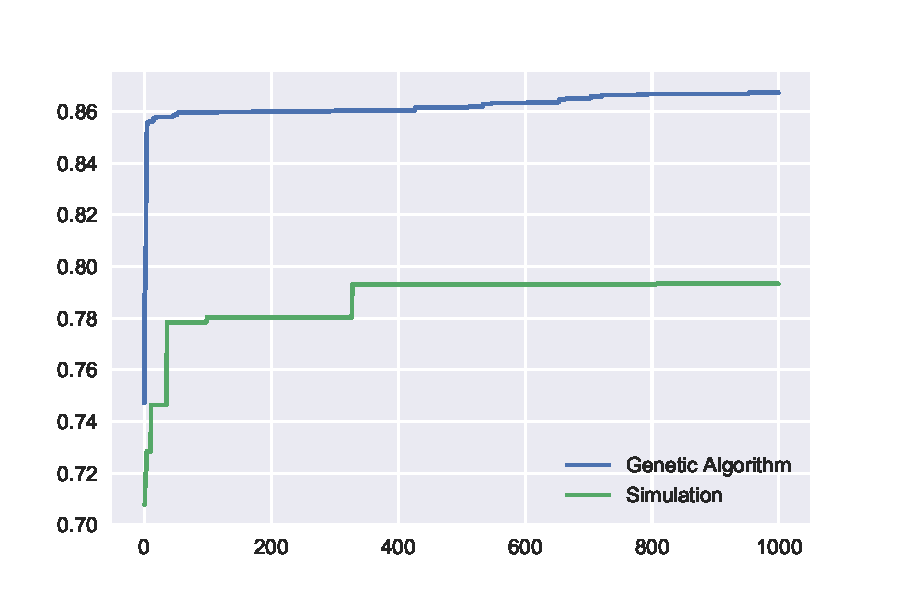
\includegraphics[scale=0.35, trim = 0 10 0 30, clip]{test_scores.pdf}
\caption{Multi-objective criterion evolution over 1000 iterations for an experimental design with 3 stimuli of 15 minutes.\label{scores}}
\end{figure}
%
\begin{figure}[t!]
\centering
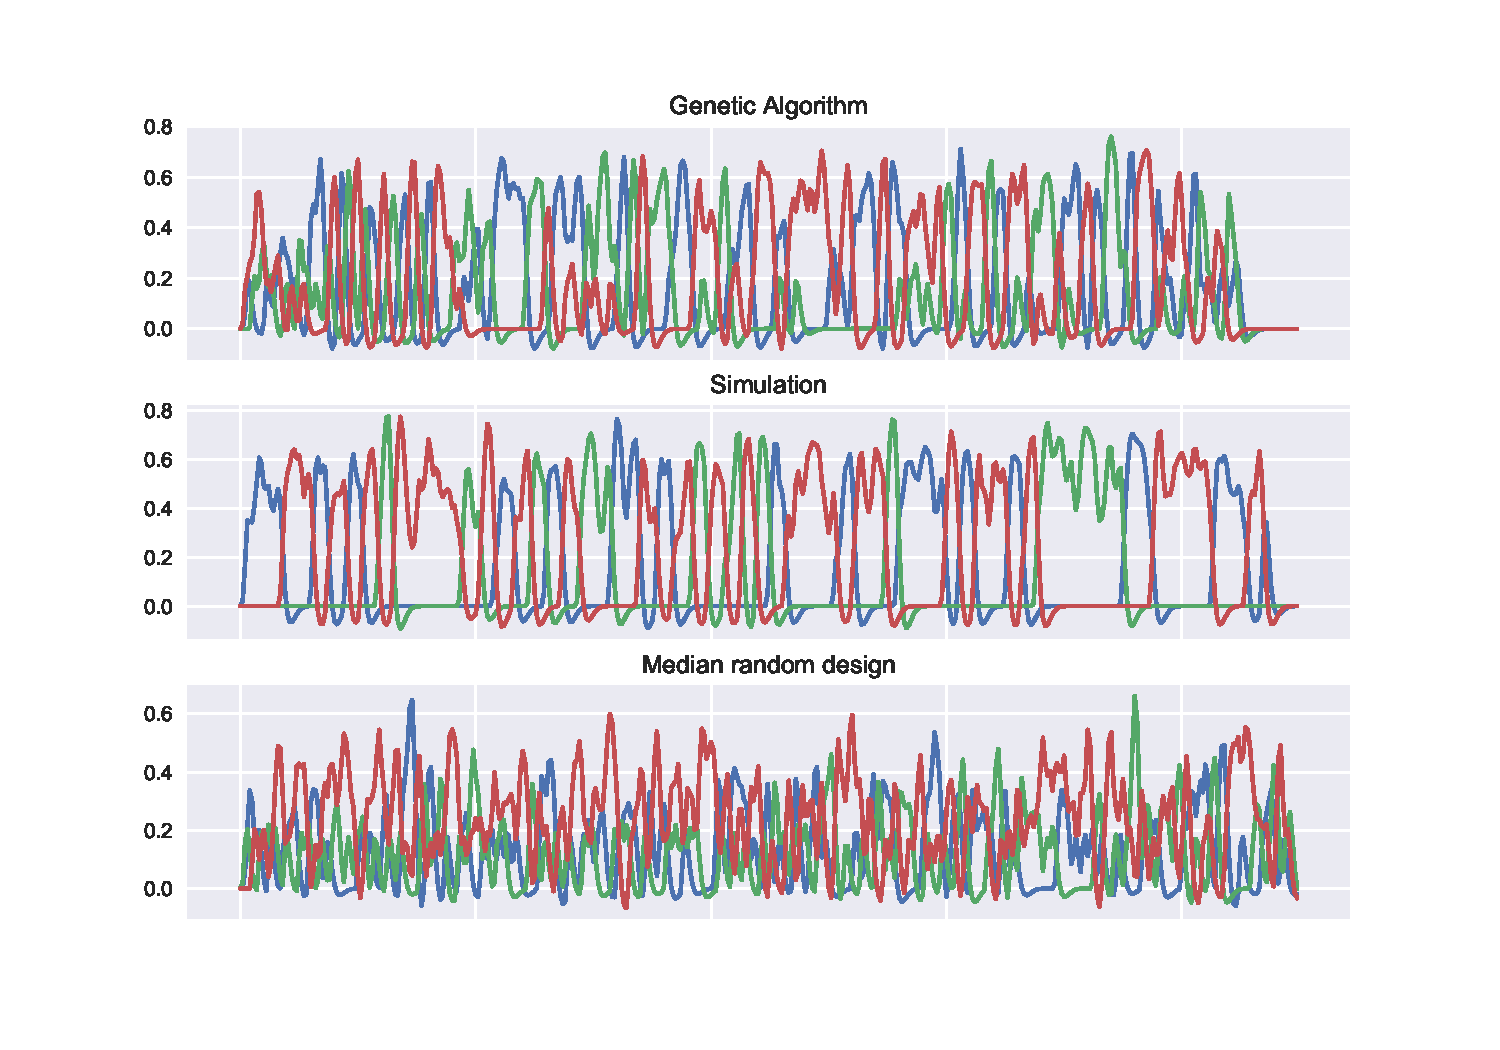
\includegraphics[scale=0.35, trim = 0 20 0 20, clip]{designs.pdf}
\caption{The resulting three designs after optimizing using the genetic algorithm, simulation based optimization, or without optimizing (median $F$).\label{designs}}
\end{figure}

\subsubsection{Simulation}

Based on the three obtained designs, we simulate fMRI data.  We
simulate data according to Equation~\ref{eq:GLM}, with $X$ the design
matrix obtained from the previous step, $\beta=(0.5,0,-0.5)^{\top}$
and $\sigma=1$.  For simplicity, we ignore the temporal
autocorrelation and analyze the data using a simple linear regression
model.  Specifically, we look at the contrasts $(1,0,0)$ and
$(1,0,-1)$, respectively corresponding to absolute effect sizes of 0.5
and 1.0.  The distribution of the resulting $T$-statistics based on
$1,000$ simulations are shown in Figure~\ref{distributions}.  We
assume a single test, thus performing statistical inference with
$\alpha=0.95$.  From the simulations, the observed statistical power
is calculated as the percentage a $T$-value exceeds the threshold,
$\#{T>t_\alpha}/10^4$.  Table~\ref{power} shows the resulting observed
statistical power. We effectively show how using \pkg{neurodesign}
significantly increases the statistical power, compared to a random
design.  Note that even though certain randomly drawn designs result
in higher power, these necessarily score lower in the other metrics,
such as predictability ($F_c$) and stimulus frequencies ($F_f$), since
none of the random designs result in a higher score for the
multi-objective criterion.
%
\begin{figure}[t!]
\centering
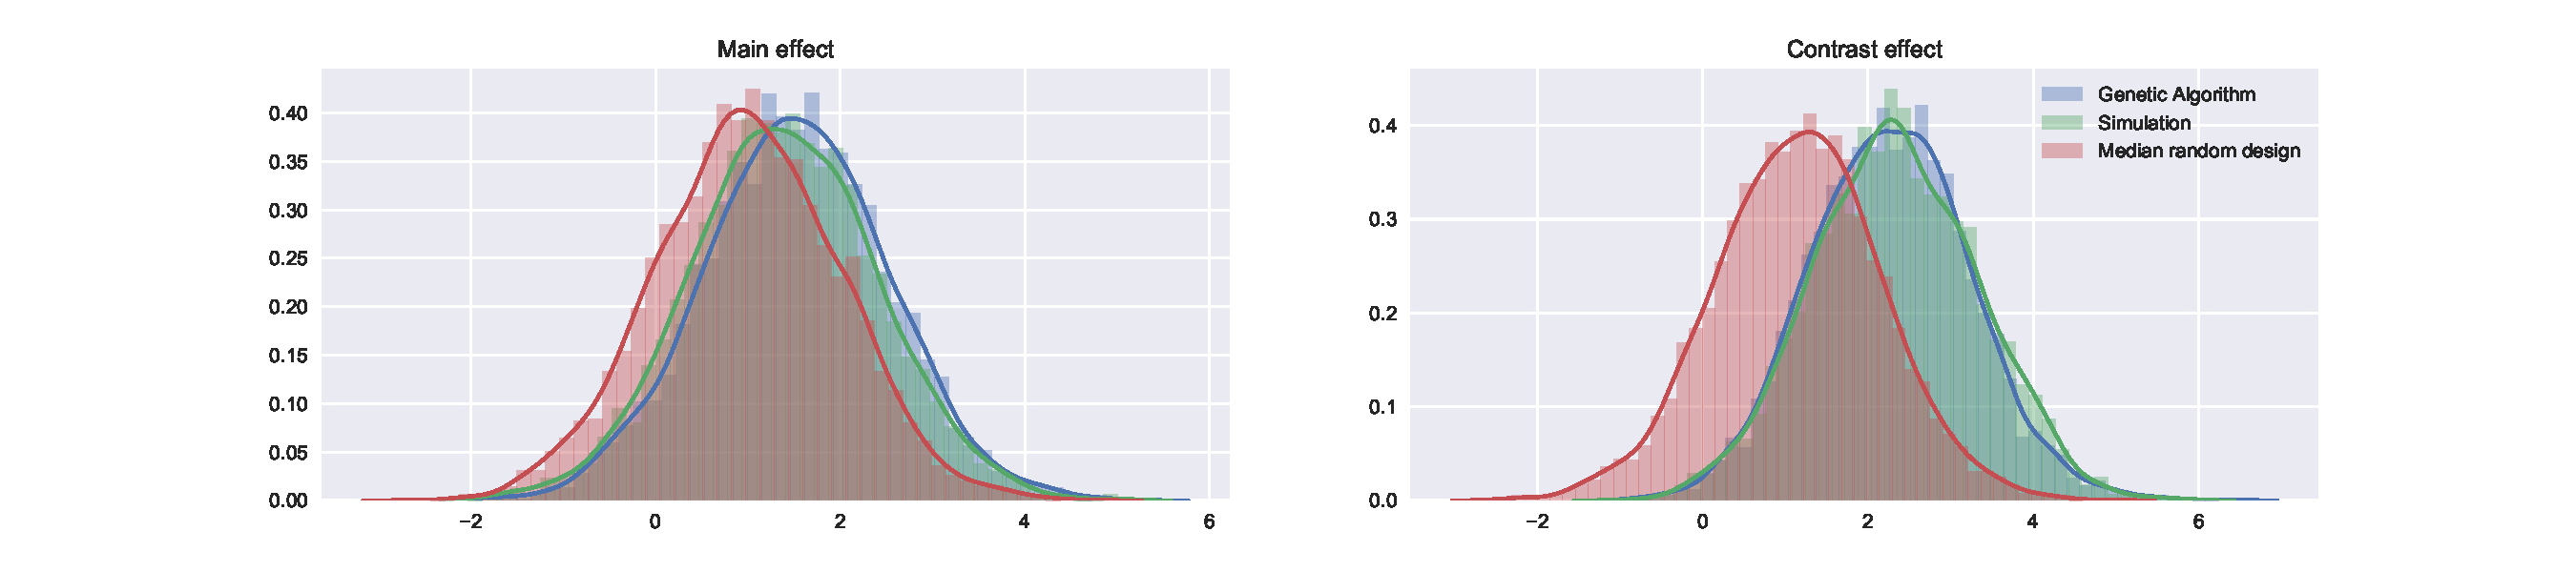
\includegraphics[scale=0.35]{distributions.pdf}
\caption{The distributions of $T$-statistics when simulating a BOLD
  signal using the three designs obtained using (1) genetic algorithm
  optimization, (2) simulation based optimization, (3) random draws
  (median $F$).\label{distributions}}
\end{figure}


 \begin{table}[t!]
     \centering
 \begin{tabular}{lcc}
 \hline   
 & {Contrast $(1,0,0)$} & {Contrast $(1,0,-1)$} \\
 \hline
 \multicolumn{1}{l}{Genetic Algorithm} &     0.45    & 0.73 \\
 \multicolumn{1}{l}{Simulation-based} &      0.40    & 0.75 \\
 \multicolumn{1}{l}{Random} &                0.26 [0.22, 0.31]    & 0.54 [0.21, 0.76] \\
\hline
 \end{tabular}
 \caption{Observed statistical power from 10000 fMRI simulations with
   3 different designs: (1) optimized using the genetic algorithm, (2)
   optimized using simulations and (3) not optimized (median [P5,
   P95]). \label{power}}
 \end{table}




\section{Discussion}\label{sec:discussion}

\subsection{Default settings}
Both the initialization of the experiment, represented by the class
experiment in the \proglang{Python} module and the main input window
in the GUI, and the genetic algorithm, represented by the class
population in the \proglang{Python} module and the settings window in
the GUI, have some default settings.  The default settings of the
\proglang{Python} module, shown in Tables~\ref{experiment}
and~\ref{population}, are pre-set to ensure a good initial
optimization, while the GUI's default settings are pre-set for short
optimization duration.  While the default settings for the GUI can
lead to a sub-optimal design, the user is warned (with a big red
text block at the top of the page) that the settings should be changed
if a good optimization is required.  We have chosen these sub-optimal
defaults for the GUI to provide a fast run through for first time
users, as well as to avoid memory and CPU overload on the server end.
For the experiment, we assume a priori that there are no rest blocks
and that the trial only consists of stimulation (no fixation cross
etc.).  There is by default no limit on the maximum number of times a
stimulus can be repeated, and the stimulus frequency is not controlled
with a hard limit.  The default resolution in the \proglang{Python}
module is 0.1 seconds, while in the GUI it is 0.25 seconds.  For the
genetic algorithm, the default settings are as follows.  The
optimization calculates the A-optimality.  In each generation, the
percentage of mutations is 1\%, the number of immigrants is 4 designs
and the size of each generation is 20 designs, as is suggested by
\citet{Kao2009}.  When generating new designs, there are 40\% blocked
designs, 40\% random designs and 20\% $m$-sequences.  Convergence is
reached when the score is stable for 1000 generations.  There are no
default settings on the number of cycles in the \proglang{Python}
module, while the GUI runs by default 10 cycles to find the maximum
$F_d$ and $F_e$ and 100 cycles for the optimization (again with a
clear message that this can be increased for better results).


\subsection{Reproducibility}
In line with the recent effort to make neuroimaging research fully
reproducible, this application makes it possible to track the exact
source of each design.  Low level reproducibility is provided by
making a script available for download with which the optimization can
be regenerated.  Running this script in \proglang{Python}, given that
the required libraries are installed, will repeat the analysis.
However, this script will repeat the analysis but does not guarantee
the same results as the specific configuration of the computer on
which the analysis is run can influence the results.

Higher level reproducibility, that guarantees replicability not only
of the analysis but also of the results, is possible with the use of
Docker containers, which is a small piece of software that emulates a
given computational configuration (operating system, libraries,
\proglang{Python} packages, \ldots).  Based on the model presented by
BIDS-apps \citep{Gorgolewski2016-wg}, our analyses run in Docker
containers that are open-source and available for download at
\url{https://hub.docker.com/r/neuropower/neuropower/}.  Running the
following command in a terminal will replicate the analysis that has
been performed through the GUI.
%%
\begin{CodeChunk}
\begin{CodeInput}
$ docker run -v /location_where_the_script_is/:/local \
>   -it neuropower/neuropower Python /local/name_of_the_script.py
\end{CodeInput}
\end{CodeChunk}
%
This use of Docker containers is not only well suited for
reproducibility of the GUI, but also allows the replication of results
from a \proglang{Python} script (given that a random seed is set). The
source code for the GUI and deployment information is available at
\url{https://github.com/neuropower/neuropower-web}.

\section{Conclusion}\label{sec:conclusion}

We present a toolbox for optimizing fMRI designs.  The toolbox is an
extension of currently available toolboxes, allowing for more complex
design and better control and optimization of timing of stimuli.  The
toolbox is available through different modalities: a user-friendly GUI
accessible at \url{http://www.neuropowertools.org} and a
\proglang{Python} package.  The code is available on
\url{https://www.github.com/neuropower}.

\section*{Acknowledgments}

This work was supported by the Laura and John Arnold Foundation.
J.D.\ has received funding from the European Unions Horizon 2020
research and innovation programme under the Marie Sklodowska-Curie
grant agreement No.~706561.

\bibliography{ref}
\end{document}
